%!TeX program = xelatex
%Do not change
\documentclass[12pt, oneside]{article}
\usepackage{amssymb,amsmath}
\usepackage[margin=1in]{geometry}
\usepackage{textpos}
\usepackage{float}
\usepackage{booktabs}
%\usepackage{color}
\usepackage{graphicx}
\usepackage[inter-unit-product =\cdot]{siunitx}
\let\DeclareUSUnit\DeclareSIUnit
\let\US\SI
\DeclareUSUnit\inch{in}
\DeclareUSUnit\foot{ft}
\DeclareUSUnit\mile{mi}
\DeclareUSUnit\foot{ft}
\DeclareUSUnit\slug{slug}
\DeclareUSUnit\pound{lb}
\DeclareUSUnit\psi{psi}
\DeclareUSUnit\Msi{Msi}
\DeclareUSUnit\ksi{ksi}

%\usepackage{tikz}
%\usetikzlibrary{positioning}
%\usepackage{tikz-3dplot}
%\usepackage{pgfopts}
%\usepackage{wasysym}
%\usepackage{stanli}

% You may add the packages you need here
\begin{document}

%TODO change numbers in problems
\begin{textblock*}{4cm}(-1.7cm,-2.3cm)
\noindent {\scriptsize AE333 Spring 2021}
\end{textblock*}

%Do not modify other than putting your name where stated
\begin{textblock*}{8cm}(12.5cm,-1cm)
\noindent {Name: }
\end{textblock*}
%Do not modify other than typing your acknowledgement where stated
\begin{textblock*}{13.5cm}(-1.7cm,-1.8cm)
%\noindent \textit{\footnotesize Acknowledgement: Your acknowledgement for collaboration and other sources goes here. }
\end{textblock*}

\vspace{1cm}

%Do not modify other than typing the homework number after #
\begin{center}
\textbf{\Large Homework 4}

\textbf{Due 1 October 2021}
\end{center}

\begin{enumerate}
	\item %p5-1
		Determine the internal torque at each section and sketch the shear stress on a volume element at $A$, $B$, $C$, and $D$.
		\begin{figure}[H]
			\centering
			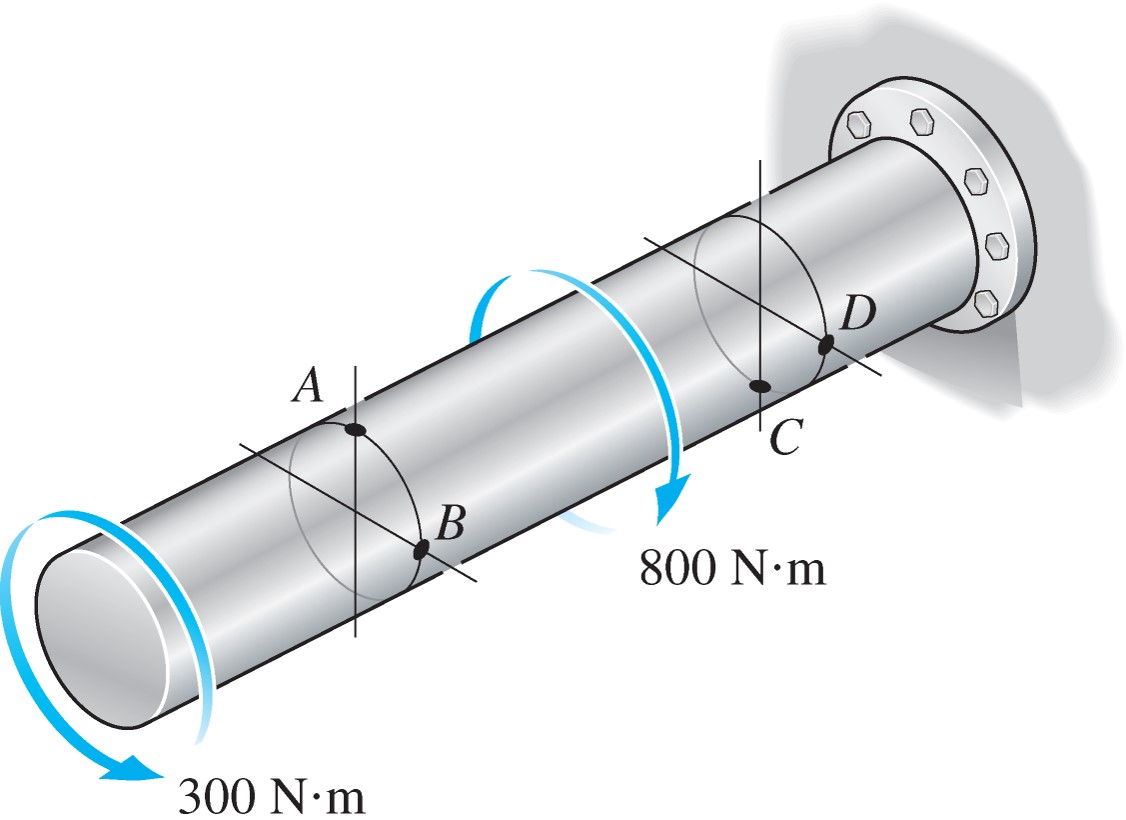
\includegraphics[width=0.6\linewidth]{p5-1}
		\end{figure}
	
	\item %5-28
		The drive shaft $AB$ is to be designed as a thin-walled tube.
		The engine delivers 150 hp while the shaft turns 1000 rpm.
		Find the minimum thickness of the shaft's wall for an outer diameter of $\US{2.5}{in}$ if the allowable shear stress is $\tau_{allow}=\US{6.0}{ksi}$.
		\begin{figure}[H]
			\centering
			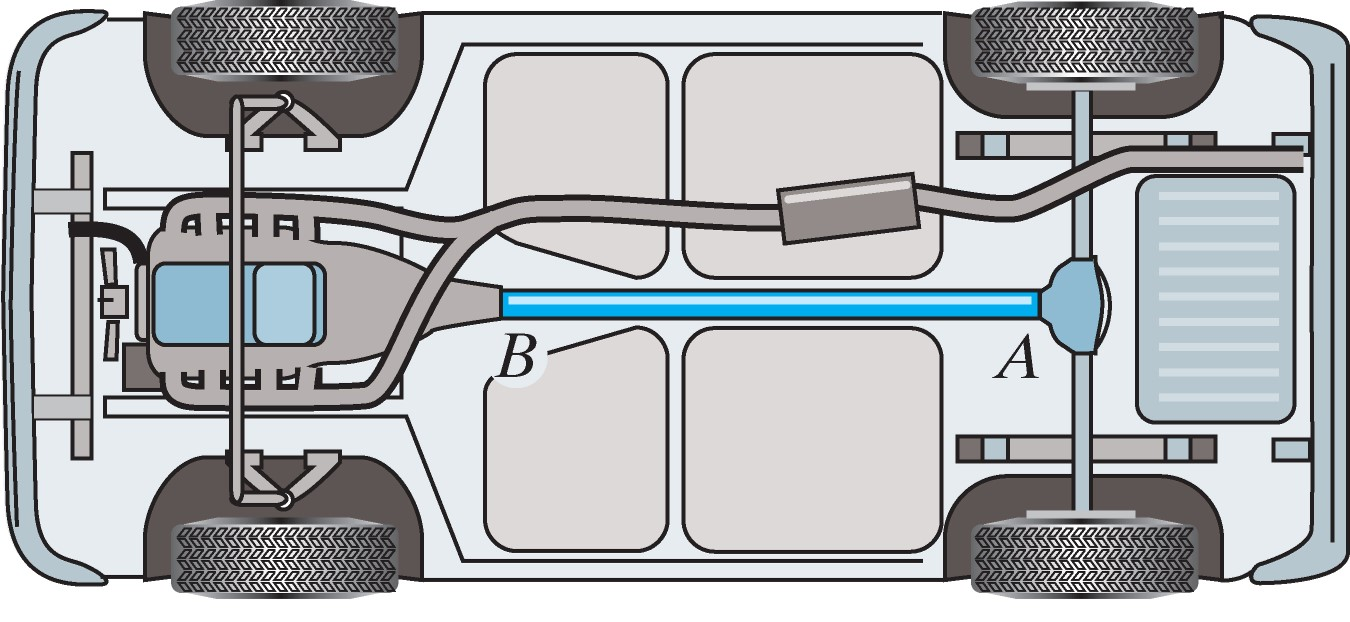
\includegraphics[width=0.6\linewidth]{5-28}
		\end{figure}
		\newpage

	\item %5-64
		The soil mixer shown is connected to an A-36 steel tubular shaft with an inside diameter of $\US{1.5}{in}$ and an outside diameter of $\US{3.0}{in}$.
		Determine the angle of twist at $A$ relative to $B$ and the absolute maximum shear stress for the torque shown.
		\begin{figure}[H]
			\centering
			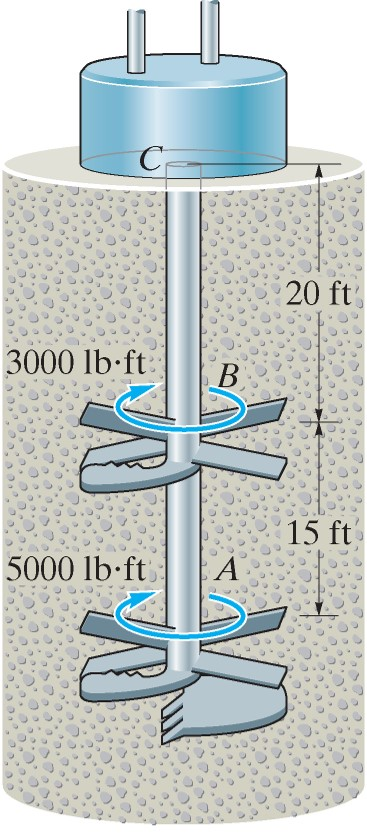
\includegraphics[width=0.2\linewidth]{5-64}
		\end{figure}

	\item %5-69
		The A-36 Steel bolt shown is tightened such that there is a reactive torque on the shank.
		The reactive torque is expressed as $t = \SI[number-math-rm = \mathnormal, parse-numbers = false]{kx^2 }{N.m/m}$ for $x$ in meters.
		If a torque of $T=\SI{45 }{N.m}$ is applied to the bold head find the value of the constant $k$ and the amount of twist in the shank.
		Assume the shank has a radius of $\SI{5 }{mm}$
		\begin{figure}[H]
			\centering
			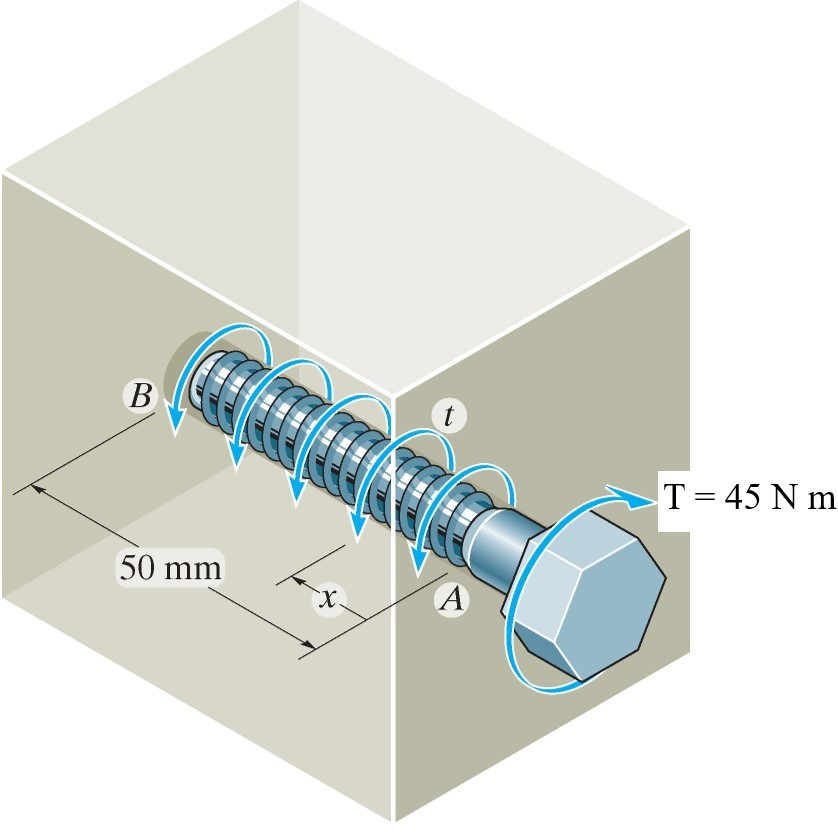
\includegraphics[width=0.6\linewidth]{5-69}
		\end{figure}

	\item %5-86
		The aluminum alloy tube (2014-T6, outside) is bonded to an A-36 steel rod (inside) as shown.
		If a torque of $\SI{7 }{kN.m}$ is applied find the maximum shear stress in each material and plot the shear stress as a function of radial position.
		\begin{figure}[H]
			\centering
			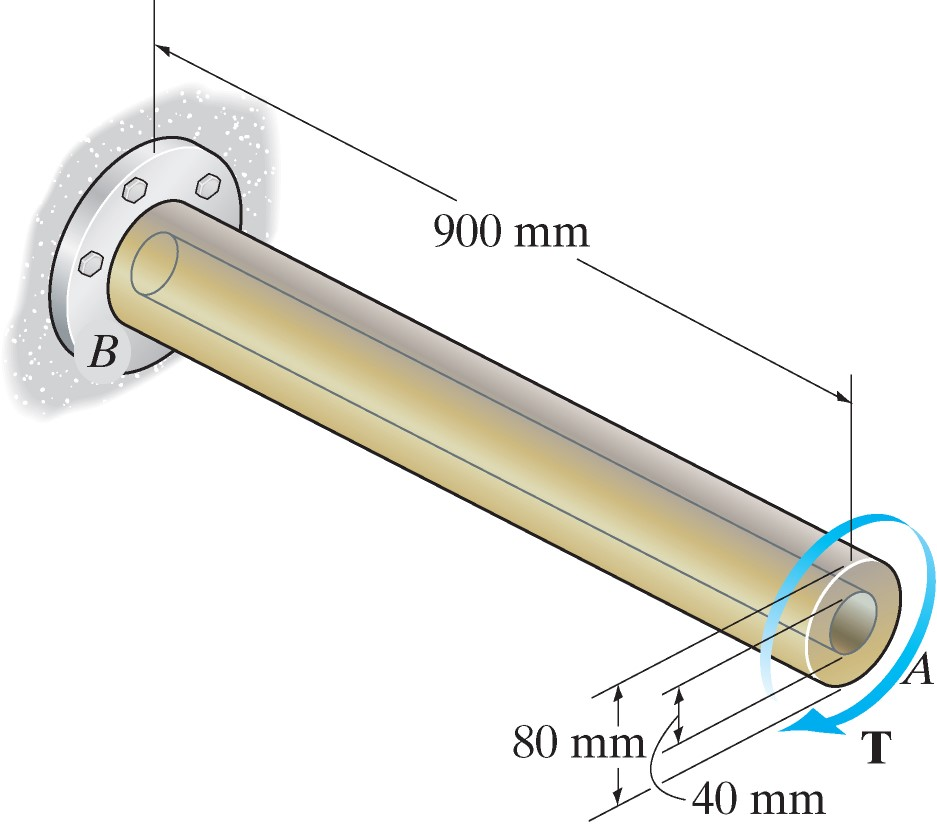
\includegraphics[width=0.6\linewidth]{5-86}
		\end{figure}

	\item %5-109
		For an arbitrary maximum shear stress, compare the torque carrying capacity between two cross-sectional shapes: the circular tube shown (inside) and the rounded rectangular tube (outside) shown.
		For both cases the wall thickness is $\US{0.1}{in}$
		\begin{figure}[H]
			\centering
			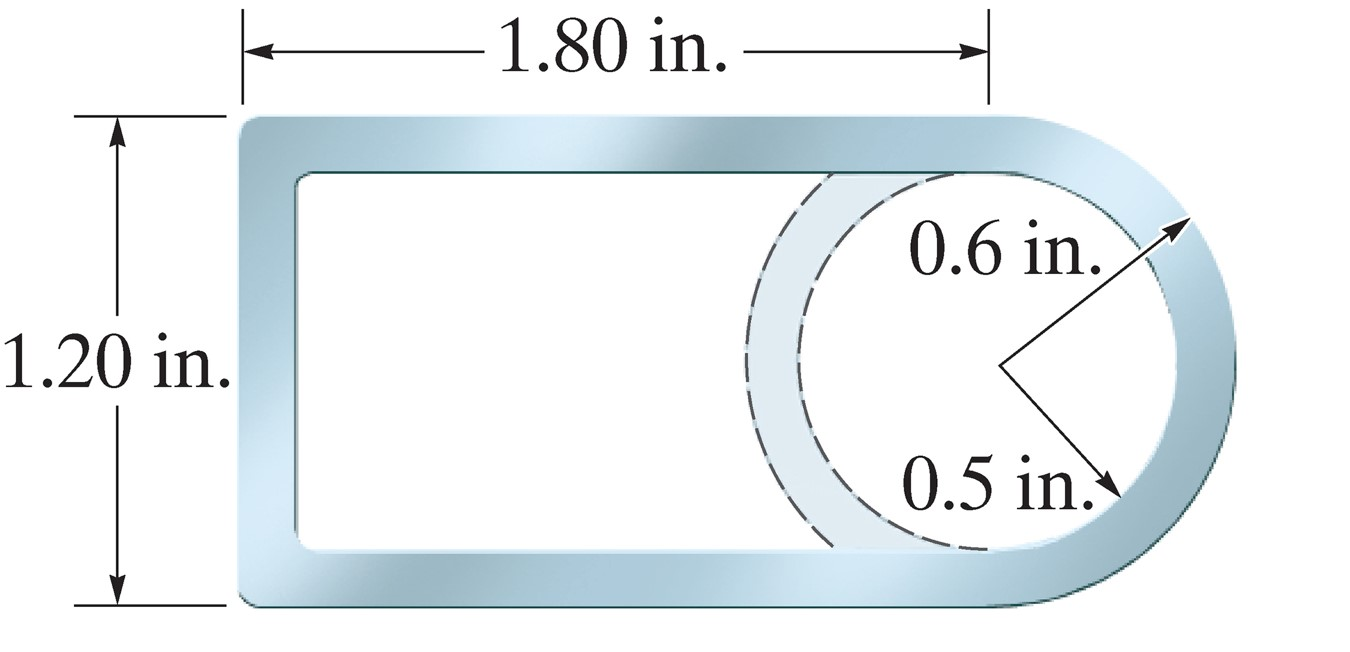
\includegraphics[width=0.6\linewidth]{5-109}
		\end{figure}

\end{enumerate}
\end{document}
